% 2012 年北京卷理科第 5 题：Rt△ABC 中 ∠ACB=90°，CD⊥AB 于 D，
% 以 BD 为直径的圆与 BC 交于 E。
% 来源 PDF：普通高考/2012/2012北京理.pdf，第 1 页（印面 717）左栏。
% 按 A(0,3)、B(4,0)、C(0,0) 的实际比例作图：D(1.44,1.92)，E(1.44,0)，
% 圆心 (2.72,0.96)，半径 1.6；只画出 BC 上方的圆弧。
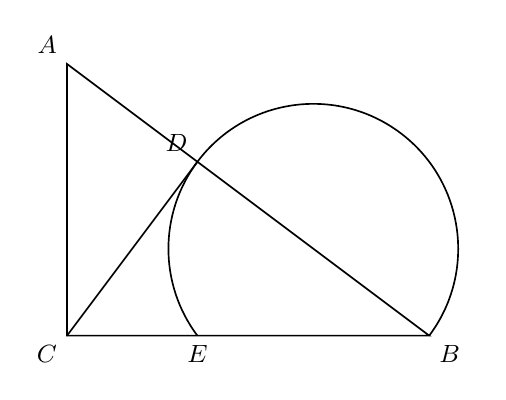
\begin{tikzpicture}[scale=1.15, semithick, font=\small]
  \coordinate (A) at (0,3);
  \coordinate (B) at (4,0);
  \coordinate (C) at (0,0);
  \coordinate (D) at (1.44,1.92);
  \coordinate (E) at (1.44,0);
  \draw (A) -- (C) -- (B) -- cycle;
  \draw (C) -- (D);
  \draw (4,0) arc[start angle=-36.87, end angle=216.87, radius=1.6];
  \node[above left] at (A) {$A$};
  \node[below left] at (C) {$C$};
  \node[below right] at (B) {$B$};
  \node[above left] at (D) {$D$};
  \node[below] at (E) {$E$};
\end{tikzpicture}
